\documentclass{standalone}
\usepackage{tikz}
\usetikzlibrary{patterns, positioning}
\usepackage[sfdefault]{ClearSans} %% option 'sfdefault' activates Clear Sans as the default text font
\usepackage[T1]{fontenc}

\begin{document}
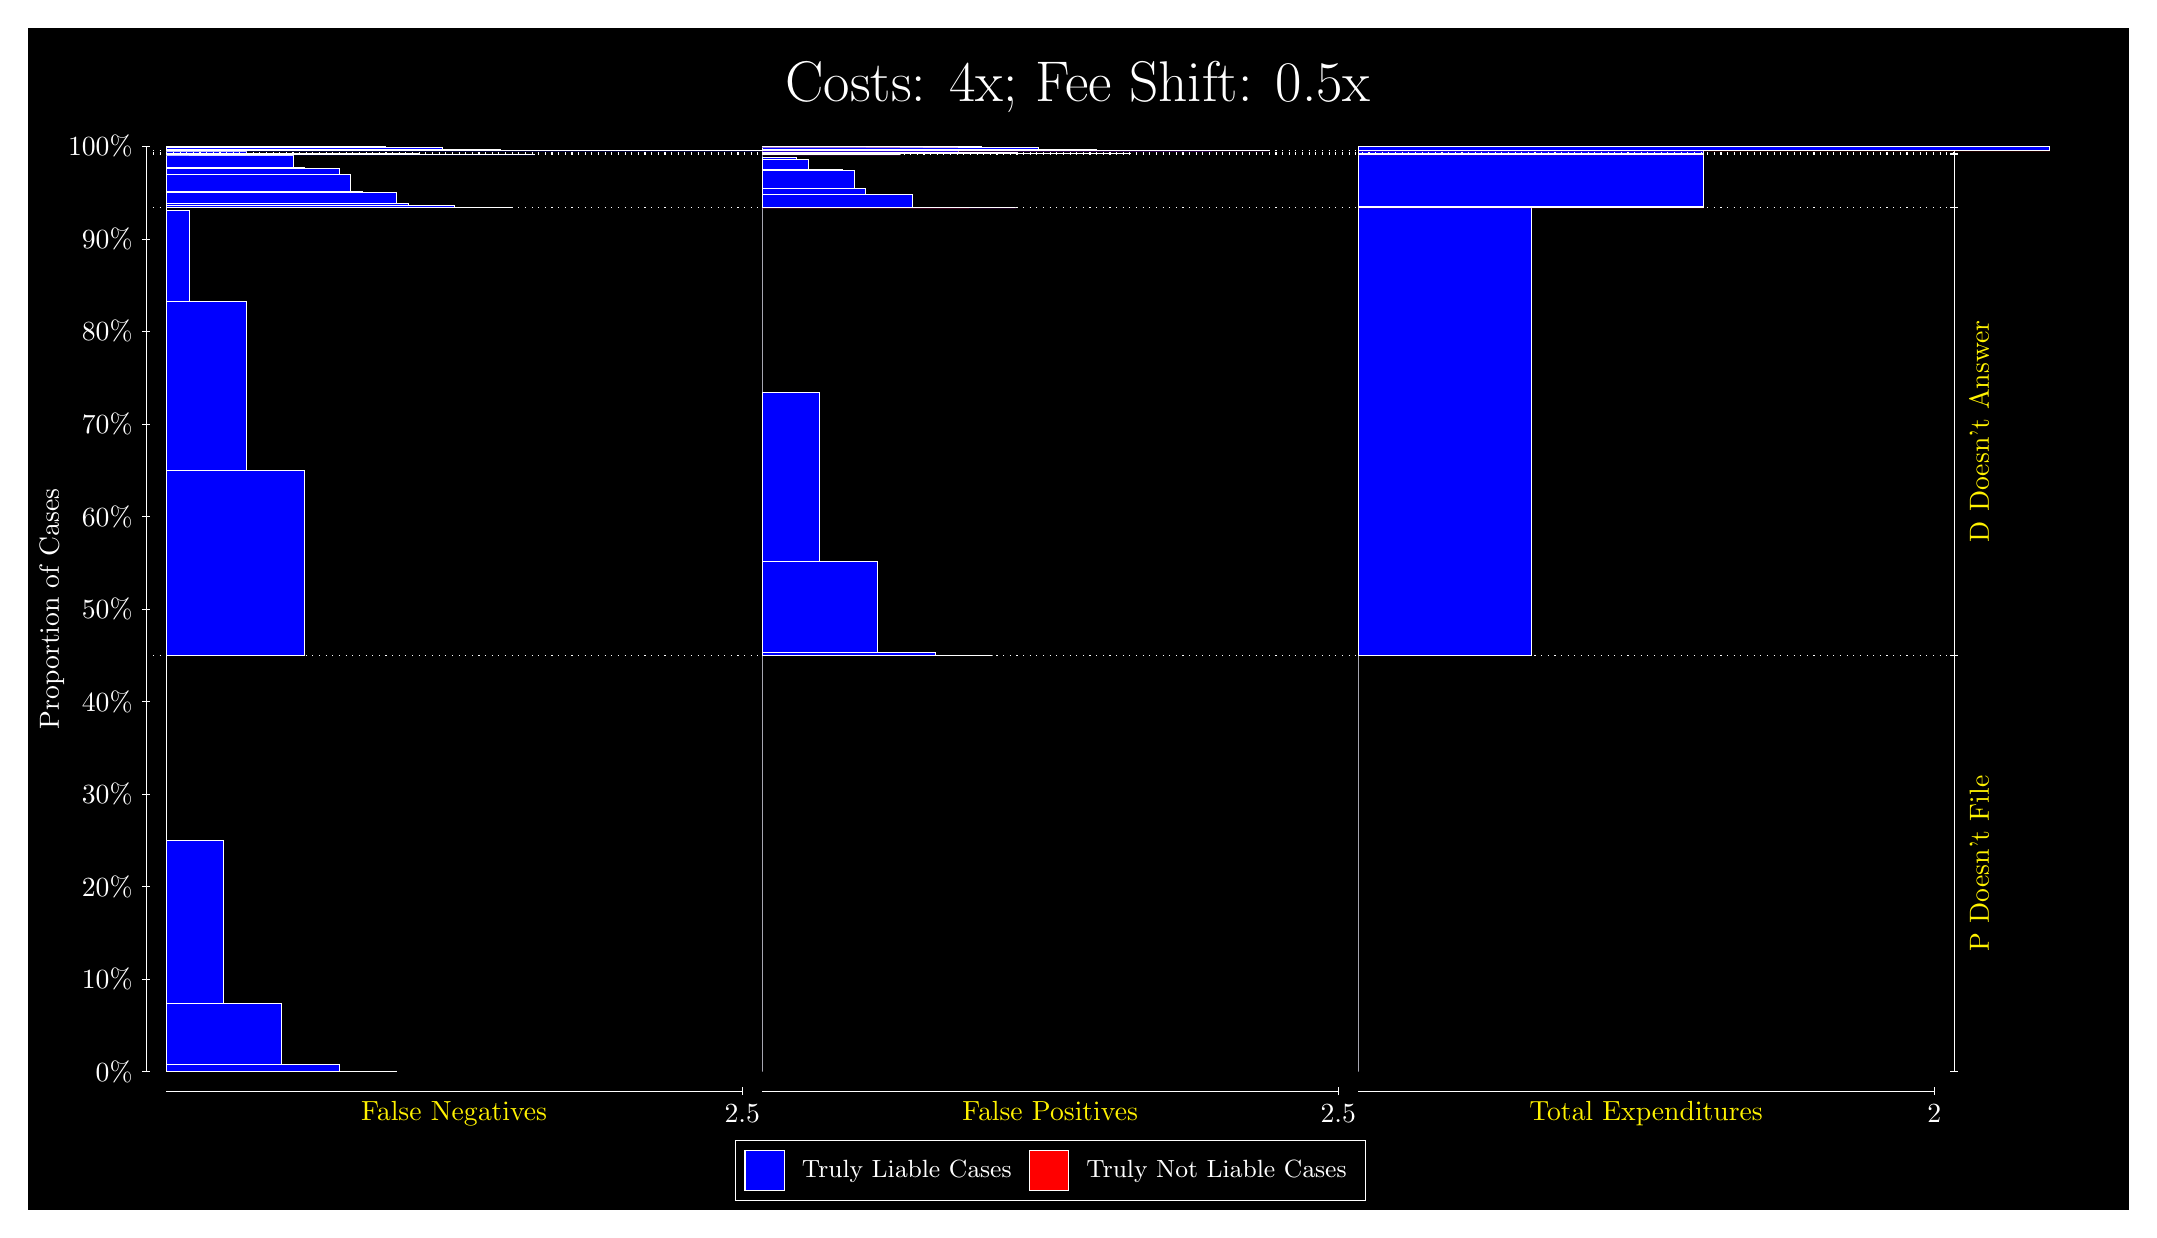
\begin{tikzpicture}
\draw[fill=black] (0,0) rectangle (26.667,15);
\draw[text=white] (0,13.5) rectangle (26.667,15) node[midway] {\huge Costs: 4x; Fee Shift: 0.5x};
\draw[white, very thin] (1.5,1.75) -- (1.5,13.5);
\node[rotate=90, text=white, anchor=center] at (0.3, 7.625) {Proportion of Cases};
\draw[white, very thin] (1.45,1.75) -- (1.55,1.75);
\node[text=white, anchor=east] at (1.45, 1.75) {0\%};
\draw[white, very thin] (1.45,2.925) -- (1.55,2.925);
\node[text=white, anchor=east] at (1.45, 2.925) {10\%};
\draw[white, very thin] (1.45,4.1) -- (1.55,4.1);
\node[text=white, anchor=east] at (1.45, 4.1) {20\%};
\draw[white, very thin] (1.45,5.275) -- (1.55,5.275);
\node[text=white, anchor=east] at (1.45, 5.275) {30\%};
\draw[white, very thin] (1.45,6.45) -- (1.55,6.45);
\node[text=white, anchor=east] at (1.45, 6.45) {40\%};
\draw[white, very thin] (1.45,7.625) -- (1.55,7.625);
\node[text=white, anchor=east] at (1.45, 7.625) {50\%};
\draw[white, very thin] (1.45,8.8) -- (1.55,8.8);
\node[text=white, anchor=east] at (1.45, 8.8) {60\%};
\draw[white, very thin] (1.45,9.975) -- (1.55,9.975);
\node[text=white, anchor=east] at (1.45, 9.975) {70\%};
\draw[white, very thin] (1.45,11.15) -- (1.55,11.15);
\node[text=white, anchor=east] at (1.45, 11.15) {80\%};
\draw[white, very thin] (1.45,12.325) -- (1.55,12.325);
\node[text=white, anchor=east] at (1.45, 12.325) {90\%};
\draw[white, very thin] (1.45,13.5) -- (1.55,13.5);
\node[text=white, anchor=east] at (1.45, 13.5) {100\%};

\draw[white, very thin] (24.457,1.75) -- (24.457,13.5);
\draw[white, very thin] (24.407,1.75) -- (24.507,1.75);
\node[anchor=west] at (24.407, 1.75) {};
\draw[white, very thin] (24.407,7.037) -- (24.507,7.037);
\node[anchor=west] at (24.407, 7.037) {};
\draw[white, very thin] (24.407,12.723) -- (24.507,12.723);
\node[anchor=west] at (24.407, 12.723) {};
\draw[white, very thin] (24.407,13.394) -- (24.507,13.394);
\node[anchor=west] at (24.407, 13.394) {};
\draw[white, very thin] (24.407,13.415) -- (24.507,13.415);
\node[anchor=west] at (24.407, 13.415) {};
\draw[white, very thin] (24.407,13.446) -- (24.507,13.446);
\node[anchor=west] at (24.407, 13.446) {};
\draw[white, very thin] (24.407,13.5) -- (24.507,13.5);
\node[anchor=west] at (24.407, 13.5) {};

\draw[white, very thin, fill=blue] (1.75,1.75) rectangle (4.6775,1.7509);
\draw[white, very thin, fill=blue] (1.75,1.7509) rectangle (3.9457,1.8467);
\draw[white, very thin, fill=blue] (1.75,1.8467) rectangle (3.2138,2.6206);
\draw[white, very thin, fill=blue] (1.75,2.6206) rectangle (2.4819,4.6898);
\draw[white, very thin, fill=red] (1.75,4.6898) rectangle (1.75,4.6898);
\draw[white, very thin, fill=blue] (1.75,4.6898) rectangle (1.75,7.037);
\draw[white, very thin, fill=blue] (1.75,7.037) rectangle (3.5065,9.3847);
\draw[white, very thin, fill=blue] (1.75,9.3847) rectangle (2.7746,11.529);
\draw[white, very thin, fill=blue] (1.75,11.529) rectangle (2.0428,12.684);
\draw[white, very thin, fill=red] (1.75,12.684) rectangle (1.75,12.684);
\draw[white, very thin, fill=blue] (1.75,12.684) rectangle (1.75,12.723);
\draw[white, very thin, fill=blue] (1.75,12.723) rectangle (6.1413,12.724);
\draw[white, very thin, fill=blue] (1.75,12.724) rectangle (5.5558,12.724);
\draw[white, very thin, fill=blue] (1.75,12.724) rectangle (5.4094,12.754);
\draw[white, very thin, fill=blue] (1.75,12.754) rectangle (4.9703,12.755);
\draw[white, very thin, fill=blue] (1.75,12.755) rectangle (4.8239,12.782);
\draw[white, very thin, fill=blue] (1.75,12.782) rectangle (4.6775,12.912);
\draw[white, very thin, fill=blue] (1.75,12.912) rectangle (4.2384,12.924);
\draw[white, very thin, fill=blue] (1.75,12.924) rectangle (4.092,13.148);
\draw[white, very thin, fill=blue] (1.75,13.148) rectangle (3.9457,13.224);
\draw[white, very thin, fill=blue] (1.75,13.224) rectangle (3.5065,13.231);
\draw[white, very thin, fill=blue] (1.75,13.231) rectangle (3.3602,13.391);
\draw[white, very thin, fill=blue] (1.75,13.391) rectangle (3.2138,13.392);
\draw[white, very thin, fill=blue] (1.75,13.392) rectangle (2.7746,13.392);
\draw[white, very thin, fill=blue] (1.75,13.392) rectangle (2.6283,13.394);
\draw[white, very thin, fill=blue] (1.75,13.394) rectangle (2.0428,13.394);
\draw[white, very thin, fill=red] (1.75,13.394) rectangle (1.75,13.394);
\draw[white, very thin, fill=blue] (1.75,13.394) rectangle (6.4341,13.394);
\draw[white, very thin, fill=blue] (1.75,13.394) rectangle (5.7022,13.4);
\draw[white, very thin, fill=blue] (1.75,13.4) rectangle (4.9703,13.412);
\draw[white, very thin, fill=blue] (1.75,13.412) rectangle (4.2384,13.415);
\draw[white, very thin, fill=blue] (1.75,13.415) rectangle (3.5065,13.415);
\draw[white, very thin, fill=red] (1.75,13.415) rectangle (1.75,13.415);
\draw[white, very thin, fill=blue] (1.75,13.415) rectangle (3.5065,13.416);
\draw[white, very thin, fill=blue] (1.75,13.416) rectangle (2.7746,13.433);
\draw[white, very thin, fill=blue] (1.75,13.433) rectangle (2.0428,13.446);
\draw[white, very thin, fill=red] (1.75,13.446) rectangle (1.75,13.446);
\draw[white, very thin, fill=blue] (1.75,13.446) rectangle (1.75,13.446);
\draw[white, very thin, fill=blue] (1.75,13.446) rectangle (9.9471,13.446);
\draw[white, very thin, fill=blue] (1.75,13.446) rectangle (9.2152,13.446);
\draw[white, very thin, fill=blue] (1.75,13.446) rectangle (8.4834,13.447);
\draw[white, very thin, fill=blue] (1.75,13.447) rectangle (7.7515,13.45);
\draw[white, very thin, fill=blue] (1.75,13.45) rectangle (7.4587,13.45);
\draw[white, very thin, fill=blue] (1.75,13.45) rectangle (7.0196,13.45);
\draw[white, very thin, fill=blue] (1.75,13.45) rectangle (6.7268,13.451);
\draw[white, very thin, fill=blue] (1.75,13.451) rectangle (6.2877,13.451);
\draw[white, very thin, fill=blue] (1.75,13.451) rectangle (5.9949,13.46);
\draw[white, very thin, fill=blue] (1.75,13.46) rectangle (5.2631,13.487);
\draw[white, very thin, fill=blue] (1.75,13.487) rectangle (4.5312,13.499);
\draw[white, very thin, fill=blue] (1.75,13.499) rectangle (3.7993,13.5);
\draw[white, very thin, fill=blue] (1.75,13.5) rectangle (3.0674,13.5);
\draw[white, very thin, fill=blue] (1.75,13.5) rectangle (2.3355,13.5);
\draw[white, very thin, fill=red] (1.75,13.5) rectangle (1.75,13.5);
\draw[white, very thin, fill=red] (9.3189,1.75) rectangle (9.3189,1.75);
\draw[white, very thin, fill=blue] (9.3189,1.75) rectangle (9.3189,7.037);
\draw[white, very thin, fill=red] (9.3189,7.037) rectangle (12.246,7.037);
\draw[white, very thin, fill=blue] (9.3189,7.037) rectangle (12.246,7.037);
\draw[white, very thin, fill=blue] (9.3189,7.037) rectangle (11.515,7.0768);
\draw[white, very thin, fill=blue] (9.3189,7.0768) rectangle (10.783,8.2318);
\draw[white, very thin, fill=blue] (9.3189,8.2318) rectangle (10.051,10.376);
\draw[white, very thin, fill=blue] (9.3189,10.376) rectangle (9.3189,12.723);
\draw[white, very thin, fill=red] (9.3189,12.723) rectangle (12.539,12.723);
\draw[white, very thin, fill=blue] (9.3189,12.723) rectangle (12.539,12.723);
\draw[white, very thin, fill=red] (9.3189,12.723) rectangle (11.954,12.723);
\draw[white, very thin, fill=blue] (9.3189,12.723) rectangle (11.954,12.725);
\draw[white, very thin, fill=blue] (9.3189,12.725) rectangle (11.807,12.725);
\draw[white, very thin, fill=red] (9.3189,12.725) rectangle (11.368,12.725);
\draw[white, very thin, fill=blue] (9.3189,12.725) rectangle (11.368,12.726);
\draw[white, very thin, fill=blue] (9.3189,12.726) rectangle (11.222,12.886);
\draw[white, very thin, fill=blue] (9.3189,12.886) rectangle (11.075,12.893);
\draw[white, very thin, fill=blue] (9.3189,12.893) rectangle (10.636,12.969);
\draw[white, very thin, fill=blue] (9.3189,12.969) rectangle (10.49,13.193);
\draw[white, very thin, fill=blue] (9.3189,13.193) rectangle (10.344,13.205);
\draw[white, very thin, fill=blue] (9.3189,13.205) rectangle (9.9044,13.335);
\draw[white, very thin, fill=blue] (9.3189,13.335) rectangle (9.758,13.362);
\draw[white, very thin, fill=blue] (9.3189,13.362) rectangle (9.6116,13.363);
\draw[white, very thin, fill=blue] (9.3189,13.363) rectangle (9.3189,13.394);
\draw[white, very thin, fill=red] (9.3189,13.394) rectangle (11.075,13.394);
\draw[white, very thin, fill=blue] (9.3189,13.394) rectangle (11.075,13.394);
\draw[white, very thin, fill=blue] (9.3189,13.394) rectangle (10.344,13.397);
\draw[white, very thin, fill=blue] (9.3189,13.397) rectangle (9.6116,13.409);
\draw[white, very thin, fill=blue] (9.3189,13.409) rectangle (9.3189,13.415);
\draw[white, very thin, fill=red] (9.3189,13.415) rectangle (14.003,13.415);
\draw[white, very thin, fill=blue] (9.3189,13.415) rectangle (14.003,13.415);
\draw[white, very thin, fill=blue] (9.3189,13.415) rectangle (13.271,13.415);
\draw[white, very thin, fill=blue] (9.3189,13.415) rectangle (12.539,13.429);
\draw[white, very thin, fill=blue] (9.3189,13.429) rectangle (11.807,13.446);
\draw[white, very thin, fill=blue] (9.3189,13.446) rectangle (11.075,13.446);
\draw[white, very thin, fill=red] (9.3189,13.446) rectangle (15.759,13.446);
\draw[white, very thin, fill=blue] (9.3189,13.446) rectangle (15.759,13.446);
\draw[white, very thin, fill=blue] (9.3189,13.446) rectangle (15.028,13.446);
\draw[white, very thin, fill=red] (9.3189,13.446) rectangle (15.028,13.446);
\draw[white, very thin, fill=blue] (9.3189,13.446) rectangle (15.028,13.446);
\draw[white, very thin, fill=blue] (9.3189,13.446) rectangle (14.296,13.447);
\draw[white, very thin, fill=red] (9.3189,13.447) rectangle (14.296,13.447);
\draw[white, very thin, fill=blue] (9.3189,13.447) rectangle (14.296,13.447);
\draw[white, very thin, fill=blue] (9.3189,13.447) rectangle (13.564,13.451);
\draw[white, very thin, fill=red] (9.3189,13.451) rectangle (13.564,13.451);
\draw[white, very thin, fill=blue] (9.3189,13.451) rectangle (13.564,13.459);
\draw[white, very thin, fill=blue] (9.3189,13.459) rectangle (12.832,13.46);
\draw[white, very thin, fill=blue] (9.3189,13.46) rectangle (12.832,13.486);
\draw[white, very thin, fill=blue] (9.3189,13.486) rectangle (12.1,13.496);
\draw[white, very thin, fill=red] (9.3189,13.496) rectangle (11.807,13.496);
\draw[white, very thin, fill=blue] (9.3189,13.496) rectangle (11.807,13.496);
\draw[white, very thin, fill=blue] (9.3189,13.496) rectangle (11.368,13.496);
\draw[white, very thin, fill=red] (9.3189,13.496) rectangle (11.075,13.496);
\draw[white, very thin, fill=blue] (9.3189,13.496) rectangle (11.075,13.496);
\draw[white, very thin, fill=blue] (9.3189,13.496) rectangle (10.636,13.496);
\draw[white, very thin, fill=blue] (9.3189,13.496) rectangle (10.344,13.499);
\draw[white, very thin, fill=blue] (9.3189,13.499) rectangle (9.6116,13.5);
\draw[white, very thin, fill=blue] (9.3189,13.5) rectangle (9.3189,13.5);
\draw[white, very thin, fill=red] (16.888,1.75) rectangle (16.888,1.75);
\draw[white, very thin, fill=blue] (16.888,1.75) rectangle (16.888,7.037);
\draw[white, very thin, fill=red] (16.888,7.037) rectangle (19.083,7.037);
\draw[white, very thin, fill=blue] (16.888,7.037) rectangle (19.083,12.723);
\draw[white, very thin, fill=red] (16.888,12.723) rectangle (21.279,12.723);
\draw[white, very thin, fill=blue] (16.888,12.723) rectangle (21.279,12.743);
\draw[white, very thin, fill=red] (16.888,12.743) rectangle (21.279,12.743);
\draw[white, very thin, fill=blue] (16.888,12.743) rectangle (21.279,13.394);
\draw[white, very thin, fill=red] (16.888,13.394) rectangle (21.279,13.394);
\draw[white, very thin, fill=blue] (16.888,13.394) rectangle (21.279,13.415);
\draw[white, very thin, fill=red] (16.888,13.415) rectangle (21.279,13.415);
\draw[white, very thin, fill=blue] (16.888,13.415) rectangle (21.279,13.446);
\draw[white, very thin, fill=red] (16.888,13.446) rectangle (25.67,13.446);
\draw[white, very thin, fill=blue] (16.888,13.446) rectangle (25.67,13.451);
\draw[white, very thin, fill=red] (16.888,13.451) rectangle (25.67,13.451);
\draw[white, very thin, fill=blue] (16.888,13.451) rectangle (25.67,13.5);
\draw[white, dotted] (1.5,7.037) -- (24.457,7.037);
\draw[white, dotted] (1.5,12.723) -- (24.457,12.723);
\draw[white, dotted] (1.5,13.394) -- (24.457,13.394);
\draw[white, dotted] (1.5,13.415) -- (24.457,13.415);
\draw[white, dotted] (1.5,13.446) -- (24.457,13.446);
\draw[white, very thin] (1.75,1.5) -- (9.0689,1.5);
\node[text=yellow, anchor=north] at (5.4094, 1.5) {False Negatives};
\draw[white, very thin] (9.0689,1.45) -- (9.0689,1.55);
\node[text=white, anchor=north] at (9.0689, 1.45) {2.5};

\draw[white, very thin] (9.3189,1.5) -- (16.638,1.5);
\node[text=yellow, anchor=north] at (12.978, 1.5) {False Positives};
\draw[white, very thin] (16.638,1.45) -- (16.638,1.55);
\node[text=white, anchor=north] at (16.638, 1.45) {2.5};

\draw[white, very thin] (16.888,1.5) -- (24.207,1.5);
\node[text=yellow, anchor=north] at (20.547, 1.5) {Total Expenditures};
\draw[white, very thin] (24.207,1.45) -- (24.207,1.55);
\node[text=white, anchor=north] at (24.207, 1.45) {2};

\node[text=yellow, centered, rotate=90] at (24.777, 4.3935) {P Doesn't File};
\node[text=yellow, centered, rotate=90] at (24.777, 9.8802) {D Doesn't Answer};





\draw (12.978300999999998,1.5) node[draw=none] (baseCoordinate) {};
\begin{scope}[align=center]
        \matrix[scale=0.5, draw=white, below=0.5cm of baseCoordinate, nodes={draw}, column sep=0.1cm]{
            \node[rectangle, draw, minimum width=0.5cm, minimum height=0.5cm, fill=blue] {}; &
            \node[draw=none, font=\small, text=white] (B) {Truly Liable Cases}; &
            \node[rectangle, draw, minimum width=0.5cm, minimum height=0.5cm, fill=red] {}; &
            \node[draw=none, font=\small, text=white] (B) {Truly Not Liable Cases}; \\
            };
\end{scope}

\end{tikzpicture}
\end{document}